\documentclass[tikz,border=8mm]{standalone}
\usepackage[T1]{fontenc}
\usepackage[utf8]{inputenc}
\usepackage{lmodern}
\usepackage{amsmath}
\usepackage{xcolor}
\usetikzlibrary{arrows.meta,calc,positioning}
\definecolor{TitleBlue}{HTML}{1D4F91}
\definecolor{Accent}{HTML}{1F6FFF}
\definecolor{Dark}{HTML}{2F3A44}
\definecolor{Grid}{HTML}{73808C}
\definecolor{SoftGray}{HTML}{F7F9FC}
\definecolor{L1}{HTML}{EAF2FC}
\definecolor{L2}{HTML}{F1F7EB}
\definecolor{L3}{HTML}{F8EDC8}
\definecolor{L4}{HTML}{EEE2F5}
\definecolor{Q1}{HTML}{D8E9FA}
\definecolor{Q2}{HTML}{D9EED2}
\definecolor{Q3}{HTML}{F7E7B3}
\definecolor{Q4}{HTML}{E8D4F0}
\begin{document}
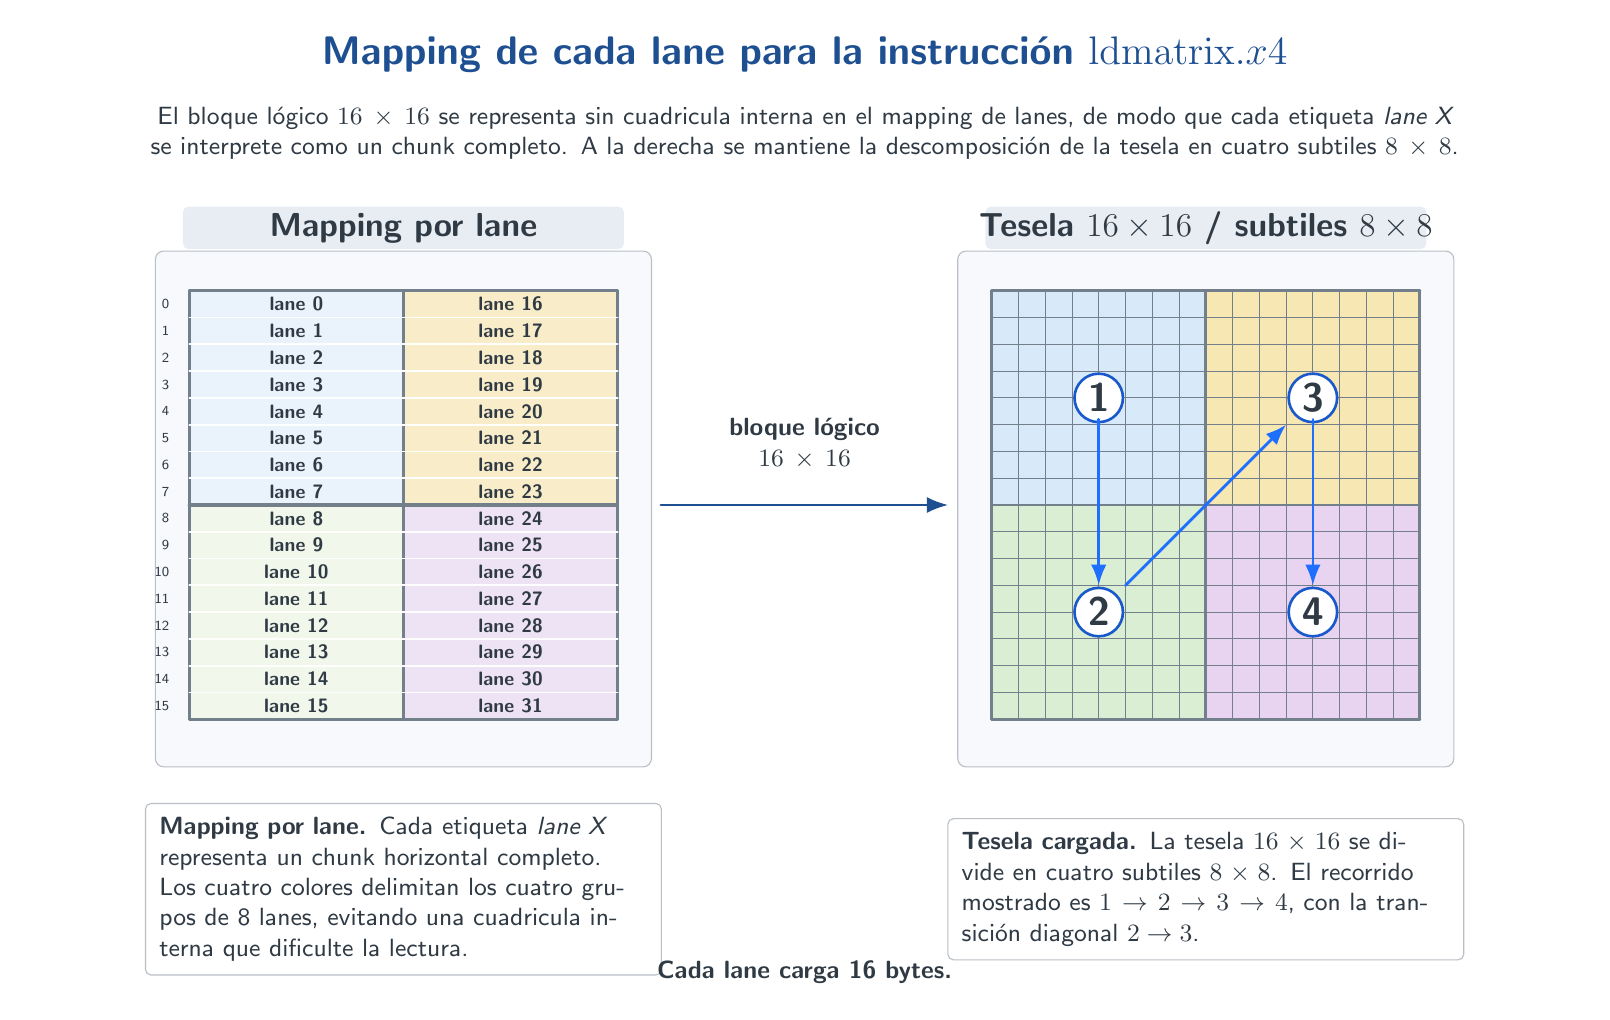
\begin{tikzpicture}[x=1cm,y=1cm,line cap=round,line join=round,>={Latex[length=2.3mm,width=1.7mm]}]
\node[font=\sffamily\bfseries\Large,text=TitleBlue,align=center,text width=19.5cm] at (8.765,11.550) {Mapping de cada lane para la instrucción $\mathrm{ldmatrix}.x4$};
\node[font=\sffamily\small,text=Dark,align=center,text width=18.8cm] at (8.765,10.550) {El bloque lógico $16\times16$ se representa sin cuadricula interna en el mapping de lanes, de modo que cada etiqueta \emph{lane X} se interprete como un chunk completo. A la derecha se mantiene la descomposición de la tesela en cuatro subtiles $8\times8$.};
\fill[TitleBlue!10,rounded corners=2pt] (0.870,9.080) rectangle (6.470,9.620);
\fill[TitleBlue!10,rounded corners=2pt] (11.060,9.080) rectangle (16.660,9.620);
\node[font=\sffamily\bfseries\large,text=Dark] at (3.670,9.350) {Mapping por lane};
\node[font=\sffamily\bfseries\large,text=Dark] at (13.860,9.350) {Tesela $16\times16$ / subtiles $8\times8$};
\node[draw=Grid!50,fill=SoftGray,rounded corners=3pt,minimum width=6.30cm,minimum height=6.55cm] at (3.670,5.780) {};
\node[draw=Grid!50,fill=SoftGray,rounded corners=3pt,minimum width=6.30cm,minimum height=6.55cm] at (13.860,5.780) {};
\fill[L1] (0.950,8.550) rectangle (3.670,5.830);
\draw[Grid,line width=1.05pt] (0.950,8.550) rectangle (3.670,5.830);
\fill[L2] (0.950,5.830) rectangle (3.670,3.110);
\draw[Grid,line width=1.05pt] (0.950,5.830) rectangle (3.670,3.110);
\fill[L3] (3.670,8.550) rectangle (6.390,5.830);
\draw[Grid,line width=1.05pt] (3.670,8.550) rectangle (6.390,5.830);
\fill[L4] (3.670,5.830) rectangle (6.390,3.110);
\draw[Grid,line width=1.05pt] (3.670,5.830) rectangle (6.390,3.110);
\draw[Grid,line width=1.12pt] (0.950,8.550) rectangle (6.390,3.110);
\draw[Grid,line width=1.12pt] (3.670,8.550) -- (3.670,3.110);
\draw[Grid,line width=1.12pt] (0.950,5.830) -- (6.390,5.830);
\node[font=\sffamily\scriptsize\bfseries,text=Dark] at (2.310,8.380) {lane 0};
\draw[white,line width=0.65pt,opacity=0.95] (0.950,8.210) -- (3.670,8.210);
\node[font=\sffamily\scriptsize\bfseries,text=Dark] at (2.310,8.040) {lane 1};
\draw[white,line width=0.65pt,opacity=0.95] (0.950,7.870) -- (3.670,7.870);
\node[font=\sffamily\scriptsize\bfseries,text=Dark] at (2.310,7.700) {lane 2};
\draw[white,line width=0.65pt,opacity=0.95] (0.950,7.530) -- (3.670,7.530);
\node[font=\sffamily\scriptsize\bfseries,text=Dark] at (2.310,7.360) {lane 3};
\draw[white,line width=0.65pt,opacity=0.95] (0.950,7.190) -- (3.670,7.190);
\node[font=\sffamily\scriptsize\bfseries,text=Dark] at (2.310,7.020) {lane 4};
\draw[white,line width=0.65pt,opacity=0.95] (0.950,6.850) -- (3.670,6.850);
\node[font=\sffamily\scriptsize\bfseries,text=Dark] at (2.310,6.680) {lane 5};
\draw[white,line width=0.65pt,opacity=0.95] (0.950,6.510) -- (3.670,6.510);
\node[font=\sffamily\scriptsize\bfseries,text=Dark] at (2.310,6.340) {lane 6};
\draw[white,line width=0.65pt,opacity=0.95] (0.950,6.170) -- (3.670,6.170);
\node[font=\sffamily\scriptsize\bfseries,text=Dark] at (2.310,6.000) {lane 7};
\node[font=\sffamily\scriptsize\bfseries,text=Dark] at (2.310,5.660) {lane 8};
\draw[white,line width=0.65pt,opacity=0.95] (0.950,5.490) -- (3.670,5.490);
\node[font=\sffamily\scriptsize\bfseries,text=Dark] at (2.310,5.320) {lane 9};
\draw[white,line width=0.65pt,opacity=0.95] (0.950,5.150) -- (3.670,5.150);
\node[font=\sffamily\scriptsize\bfseries,text=Dark] at (2.310,4.980) {lane 10};
\draw[white,line width=0.65pt,opacity=0.95] (0.950,4.810) -- (3.670,4.810);
\node[font=\sffamily\scriptsize\bfseries,text=Dark] at (2.310,4.640) {lane 11};
\draw[white,line width=0.65pt,opacity=0.95] (0.950,4.470) -- (3.670,4.470);
\node[font=\sffamily\scriptsize\bfseries,text=Dark] at (2.310,4.300) {lane 12};
\draw[white,line width=0.65pt,opacity=0.95] (0.950,4.130) -- (3.670,4.130);
\node[font=\sffamily\scriptsize\bfseries,text=Dark] at (2.310,3.960) {lane 13};
\draw[white,line width=0.65pt,opacity=0.95] (0.950,3.790) -- (3.670,3.790);
\node[font=\sffamily\scriptsize\bfseries,text=Dark] at (2.310,3.620) {lane 14};
\draw[white,line width=0.65pt,opacity=0.95] (0.950,3.450) -- (3.670,3.450);
\node[font=\sffamily\scriptsize\bfseries,text=Dark] at (2.310,3.280) {lane 15};
\node[font=\sffamily\scriptsize\bfseries,text=Dark] at (5.030,8.380) {lane 16};
\draw[white,line width=0.65pt,opacity=0.95] (3.670,8.210) -- (6.390,8.210);
\node[font=\sffamily\scriptsize\bfseries,text=Dark] at (5.030,8.040) {lane 17};
\draw[white,line width=0.65pt,opacity=0.95] (3.670,7.870) -- (6.390,7.870);
\node[font=\sffamily\scriptsize\bfseries,text=Dark] at (5.030,7.700) {lane 18};
\draw[white,line width=0.65pt,opacity=0.95] (3.670,7.530) -- (6.390,7.530);
\node[font=\sffamily\scriptsize\bfseries,text=Dark] at (5.030,7.360) {lane 19};
\draw[white,line width=0.65pt,opacity=0.95] (3.670,7.190) -- (6.390,7.190);
\node[font=\sffamily\scriptsize\bfseries,text=Dark] at (5.030,7.020) {lane 20};
\draw[white,line width=0.65pt,opacity=0.95] (3.670,6.850) -- (6.390,6.850);
\node[font=\sffamily\scriptsize\bfseries,text=Dark] at (5.030,6.680) {lane 21};
\draw[white,line width=0.65pt,opacity=0.95] (3.670,6.510) -- (6.390,6.510);
\node[font=\sffamily\scriptsize\bfseries,text=Dark] at (5.030,6.340) {lane 22};
\draw[white,line width=0.65pt,opacity=0.95] (3.670,6.170) -- (6.390,6.170);
\node[font=\sffamily\scriptsize\bfseries,text=Dark] at (5.030,6.000) {lane 23};
\node[font=\sffamily\scriptsize\bfseries,text=Dark] at (5.030,5.660) {lane 24};
\draw[white,line width=0.65pt,opacity=0.95] (3.670,5.490) -- (6.390,5.490);
\node[font=\sffamily\scriptsize\bfseries,text=Dark] at (5.030,5.320) {lane 25};
\draw[white,line width=0.65pt,opacity=0.95] (3.670,5.150) -- (6.390,5.150);
\node[font=\sffamily\scriptsize\bfseries,text=Dark] at (5.030,4.980) {lane 26};
\draw[white,line width=0.65pt,opacity=0.95] (3.670,4.810) -- (6.390,4.810);
\node[font=\sffamily\scriptsize\bfseries,text=Dark] at (5.030,4.640) {lane 27};
\draw[white,line width=0.65pt,opacity=0.95] (3.670,4.470) -- (6.390,4.470);
\node[font=\sffamily\scriptsize\bfseries,text=Dark] at (5.030,4.300) {lane 28};
\draw[white,line width=0.65pt,opacity=0.95] (3.670,4.130) -- (6.390,4.130);
\node[font=\sffamily\scriptsize\bfseries,text=Dark] at (5.030,3.960) {lane 29};
\draw[white,line width=0.65pt,opacity=0.95] (3.670,3.790) -- (6.390,3.790);
\node[font=\sffamily\scriptsize\bfseries,text=Dark] at (5.030,3.620) {lane 30};
\draw[white,line width=0.65pt,opacity=0.95] (3.670,3.450) -- (6.390,3.450);
\node[font=\sffamily\scriptsize\bfseries,text=Dark] at (5.030,3.280) {lane 31};
\node[anchor=east,font=\sffamily\tiny,text=Dark] at (0.820,8.380) {0};
\node[anchor=east,font=\sffamily\tiny,text=Dark] at (0.820,8.040) {1};
\node[anchor=east,font=\sffamily\tiny,text=Dark] at (0.820,7.700) {2};
\node[anchor=east,font=\sffamily\tiny,text=Dark] at (0.820,7.360) {3};
\node[anchor=east,font=\sffamily\tiny,text=Dark] at (0.820,7.020) {4};
\node[anchor=east,font=\sffamily\tiny,text=Dark] at (0.820,6.680) {5};
\node[anchor=east,font=\sffamily\tiny,text=Dark] at (0.820,6.340) {6};
\node[anchor=east,font=\sffamily\tiny,text=Dark] at (0.820,6.000) {7};
\node[anchor=east,font=\sffamily\tiny,text=Dark] at (0.820,5.660) {8};
\node[anchor=east,font=\sffamily\tiny,text=Dark] at (0.820,5.320) {9};
\node[anchor=east,font=\sffamily\tiny,text=Dark] at (0.820,4.980) {10};
\node[anchor=east,font=\sffamily\tiny,text=Dark] at (0.820,4.640) {11};
\node[anchor=east,font=\sffamily\tiny,text=Dark] at (0.820,4.300) {12};
\node[anchor=east,font=\sffamily\tiny,text=Dark] at (0.820,3.960) {13};
\node[anchor=east,font=\sffamily\tiny,text=Dark] at (0.820,3.620) {14};
\node[anchor=east,font=\sffamily\tiny,text=Dark] at (0.820,3.280) {15};
\fill[Q1] (11.140,8.550) rectangle (13.860,5.830);
\fill[Q2] (11.140,5.830) rectangle (13.860,3.110);
\fill[Q3] (13.860,8.550) rectangle (16.580,5.830);
\fill[Q4] (13.860,5.830) rectangle (16.580,3.110);
\draw[Grid,line width=1.08pt] (11.140,8.550) -- (11.140,3.110);
\draw[Grid,line width=0.30pt] (11.480,8.550) -- (11.480,3.110);
\draw[Grid,line width=0.30pt] (11.820,8.550) -- (11.820,3.110);
\draw[Grid,line width=0.30pt] (12.160,8.550) -- (12.160,3.110);
\draw[Grid,line width=0.30pt] (12.500,8.550) -- (12.500,3.110);
\draw[Grid,line width=0.30pt] (12.840,8.550) -- (12.840,3.110);
\draw[Grid,line width=0.30pt] (13.180,8.550) -- (13.180,3.110);
\draw[Grid,line width=0.30pt] (13.520,8.550) -- (13.520,3.110);
\draw[Grid,line width=1.08pt] (13.860,8.550) -- (13.860,3.110);
\draw[Grid,line width=0.30pt] (14.200,8.550) -- (14.200,3.110);
\draw[Grid,line width=0.30pt] (14.540,8.550) -- (14.540,3.110);
\draw[Grid,line width=0.30pt] (14.880,8.550) -- (14.880,3.110);
\draw[Grid,line width=0.30pt] (15.220,8.550) -- (15.220,3.110);
\draw[Grid,line width=0.30pt] (15.560,8.550) -- (15.560,3.110);
\draw[Grid,line width=0.30pt] (15.900,8.550) -- (15.900,3.110);
\draw[Grid,line width=0.30pt] (16.240,8.550) -- (16.240,3.110);
\draw[Grid,line width=1.08pt] (16.580,8.550) -- (16.580,3.110);
\draw[Grid,line width=1.08pt] (11.140,8.550) -- (16.580,8.550);
\draw[Grid,line width=0.30pt] (11.140,8.210) -- (16.580,8.210);
\draw[Grid,line width=0.30pt] (11.140,7.870) -- (16.580,7.870);
\draw[Grid,line width=0.30pt] (11.140,7.530) -- (16.580,7.530);
\draw[Grid,line width=0.30pt] (11.140,7.190) -- (16.580,7.190);
\draw[Grid,line width=0.30pt] (11.140,6.850) -- (16.580,6.850);
\draw[Grid,line width=0.30pt] (11.140,6.510) -- (16.580,6.510);
\draw[Grid,line width=0.30pt] (11.140,6.170) -- (16.580,6.170);
\draw[Grid,line width=1.08pt] (11.140,5.830) -- (16.580,5.830);
\draw[Grid,line width=0.30pt] (11.140,5.490) -- (16.580,5.490);
\draw[Grid,line width=0.30pt] (11.140,5.150) -- (16.580,5.150);
\draw[Grid,line width=0.30pt] (11.140,4.810) -- (16.580,4.810);
\draw[Grid,line width=0.30pt] (11.140,4.470) -- (16.580,4.470);
\draw[Grid,line width=0.30pt] (11.140,4.130) -- (16.580,4.130);
\draw[Grid,line width=0.30pt] (11.140,3.790) -- (16.580,3.790);
\draw[Grid,line width=0.30pt] (11.140,3.450) -- (16.580,3.450);
\draw[Grid,line width=1.08pt] (11.140,3.110) -- (16.580,3.110);
\node[circle,draw=Accent!80!black,line width=0.95pt,fill=white,inner sep=1.7pt,font=\sffamily\bfseries\Large,text=Dark] at (12.500,7.190) {1};
\node[circle,draw=Accent!80!black,line width=0.95pt,fill=white,inner sep=1.7pt,font=\sffamily\bfseries\Large,text=Dark] at (12.500,4.470) {2};
\node[circle,draw=Accent!80!black,line width=0.95pt,fill=white,inner sep=1.7pt,font=\sffamily\bfseries\Large,text=Dark] at (15.220,7.190) {3};
\node[circle,draw=Accent!80!black,line width=0.95pt,fill=white,inner sep=1.7pt,font=\sffamily\bfseries\Large,text=Dark] at (15.220,4.470) {4};
\draw[-Latex,Accent,line width=1.0pt] (12.500,6.918) -- (12.500,4.810);
\draw[-Latex,Accent,line width=1.0pt] (12.840,4.810) -- (14.880,6.850);
\draw[-Latex,Accent,line width=1.0pt] (15.220,6.918) -- (15.220,4.810);
\draw[-Latex,TitleBlue,line width=1.05pt] (6.940,5.830) -- (10.590,5.830);
\node[font=\sffamily\small\bfseries,text=Dark,align=center,text width=3.6cm,fill=white,inner sep=3pt] at (8.765,6.610) {bloque lógico\\$16\times16$};
\node[draw=Grid!50,fill=white,rounded corners=2pt,inner sep=5pt,text width=6.2cm,font=\sffamily\small,text=Dark,align=left] at (3.670,0.950) {\textbf{Mapping por lane.} Cada etiqueta \emph{lane X} representa un chunk horizontal completo. Los cuatro colores delimitan los cuatro grupos de 8 lanes, evitando una cuadricula interna que dificulte la lectura.};
\node[draw=Grid!50,fill=white,rounded corners=2pt,inner sep=5pt,text width=6.2cm,font=\sffamily\small,text=Dark,align=left] at (13.860,0.950) {\textbf{Tesela cargada.} La tesela $16\times16$ se divide en cuatro subtiles $8\times8$. El recorrido mostrado es $1\rightarrow2\rightarrow3\rightarrow4$, con la transición diagonal $2\rightarrow3$.};
\node[font=\sffamily\small\bfseries,text=Dark] at (8.765,-0.10) {Cada lane carga 16 bytes.};
\end{tikzpicture}
\end{document}
